\section{Results}
\label{sec:results}
\Cref{fig:retrieval} shows the evolution of retrieval results on the
{\sc dialog} and {\sc narration} validation data as function of
training steps.  Likewise \Cref{fig:triplet} shows the accuracy on the
triplet task on these two data splits. The segments for the triplet
task is based on aligned subtitles; for the retrieval task 3.2 seconds
segments are used.

\begin{figure}
  \centering
  \begin{tabular}{cc}
    Dialog & Narration \\
    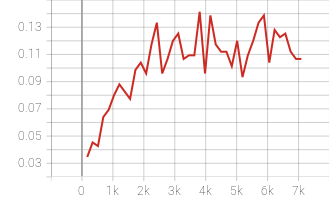
\includegraphics[scale=0.3]{val_rec10.png} & 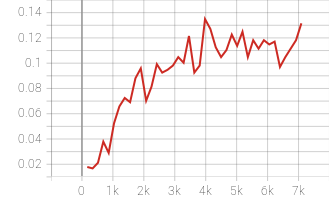
\includegraphics[scale=0.3]{valnarr_rec10.png}\\
  \end{tabular}
  \caption{Recall@10 on the retrieval task. The x-axis shows the training
    steps.}
  \label{fig:retrieval}
\end{figure}

\begin{figure}
  \centering
  \begin{tabular}{cc}
    Dialog & Narration \\
    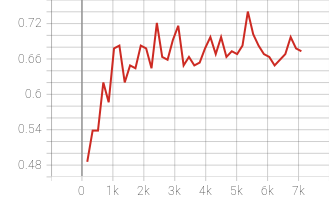
\includegraphics[scale=0.3]{val_acc3.png}  & 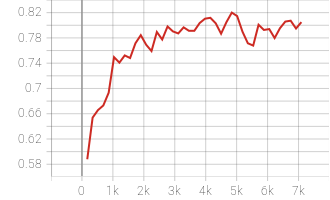
\includegraphics[scale=0.3]{valnarr_acc3.png}\\
  \end{tabular}
  \caption{Accuracy on the triplet task. The x-axis shows the training
    steps.}
  \label{fig:triplet}
\end{figure}